\documentclass[a4paper]{article}
\makeatletter
\usepackage[voffset=0in, textheight=10in]{geometry}
%[voffset=0in, textheight=10in, footskip=0]
%[margin=2cm, heightrounded, marginparwidth=3cm, marginparsep=1cm]
\usepackage{listings}
\usepackage{multicol}
\usepackage{marginnote}
\usepackage{color}
\usepackage{tikz-qtree}
\usepackage{float}
\usepackage{tikz}
\usetikzlibrary{shapes.geometric, arrows}
\makeatother
\definecolor{comment}{rgb}{0,0.6,0}
\definecolor{number}{rgb}{0.5,0.5,0.5}
\definecolor{string}{rgb}{0.58,0,0.82}
\definecolor{backcolour}{rgb}{0.95,0.95,0.92}
\tikzstyle{startstop} = [rectangle, rounded corners, minimum width=3cm, minimum height=1cm,text centered, draw=black]
\lstdefinestyle{mystyle}{
	backgroundcolor=\color{backcolour},   
	commentstyle=\color{comment},
	keywordstyle=\color{magenta},
	numberstyle=\tiny\color{number},
	stringstyle=\color{string},
	basicstyle=\footnotesize,
	breakatwhitespace=false,         
	breaklines=true,                 
	captionpos=b,                    
	keepspaces=true,                 
	numbers=left,                    
	numbersep=5pt,                  
	showspaces=false,                
	showstringspaces=false,
	showtabs=false,                  
	tabsize=2
}
\reversemarginpar
\lstset{style=mystyle}
\tikzset{edge from parent/.style=
	{draw, edge from parent path={(\tikzparentnode.south)
			-- +(0,-10pt)
			-| (\tikzchildnode)}},
	blank/.style={draw=none}}

\begin{document}
	\marginnote{Specification Section}[1cm]
	\section{Fundamentals of Programming}
		\subsection{Programming}
			\marginnote{3.1.1.1}[0cm]A data type determines what sort of datum is being stored and how it will be handled by the program. There are several built in data types common to many programming languages:
			\begin{itemize}
				\setlength\itemsep{0em}
				\item Integer: Any positive or negative whole number including zero.
					\subitem -2, -1, 0, 1, 2
				\item Real/Float: Any number with a decimal/fractional part.
					\subitem -1, $ -\frac{1}{2} $, 0, 0.543543, 1
				\item Boolean: True or False.
				\item Character: An individual character (alphanumerical or symbol).
					\subitem "a", "1", "\&"
				\item String: A sequence of characters.
					\subitem "Hello World"
				\item Date/Time: A date or time.
					\subitem 28.05.2016 12:39:40:056
				\item Records: A collection of items which be of different data types which are related.
					\subitem [ \{Name: "Nathan", age: 17\} ,\{Name: "Serena", age: 17\} ]
				\item Arrays: A collection of items of the same data type.
					\subitem [ "Ryan", "Helen", "Luke","Giorgia" ]
			\end{itemize}
			A user defined data type is a data type that is made of built-in data types (A data type that is provided within the programming language being used). In python you can write your own data types by writing type methods in C, or simply creating a class which does what you want. \\ \\
			\marginnote{3.1.1.2}[0cm]Within a program there is usually a combination of the following statement types:
			\begin{itemize}
				\setlength\itemsep{0em}
				\item Variable declaration: The process of defining a variable in terms of its data type and identifier (variable name).
				\item Constant declaration: The process of defining a constant in terms of its data type and identifier (constant name).
				\item Assignment: Giving a value to a variable or constant.
				\item Iteration: The principle of repeating processes.
				\item Selection: The principle of choosing what action to take based on certain criteria.
				\item Subroutine (AKA Procedure): A named block of code designed to carry out a specific task.
				\item Function: A subroutine which returns a value.
			\end{itemize}
			In python, all of the variables and constants are dynamically typed, meaning you don't have to worry about declaring a data type, as it is taken care of by the programming language. \\
			Within imperative programs the combining of the principles sequencing, iteration and selection are basic to all of them.\\
			Definite iteration is when a process repeats a set amount of time, for example:
			\begin{lstlisting}[language=python]
for x in range(10):
	print("hi")\end{lstlisting}
			This would print \verb|hi| 10 times. Indefinite iteration is a process that repeats until a certain condition is met. This can be done in two ways, \textit{Method 1} with the condition at the beginning, and \textit{Method 2} with the condition at the end. The implications of these two methods is that \textit{Method 2} forces the loop to be done once, whereas the loop in method one may never be done. This can be shown using an example using both methods:
			\begin{multicols}{2}
				Method 1
				\begin{lstlisting}[language=python]
x = 5
while x < 5:
	print(x)\end{lstlisting}
				
				\columnbreak
				Method 2
				\begin{lstlisting}[language=python]
x = 5
while True:
	print(x)
	if not (x<5):
		break \end{lstlisting}
				
			\end{multicols}
			\noindent
			Method one results in nothing being printed as \verb|x| starts as \verb|5| so \verb|x<5| \verb|False|, so the loop never runs, so \verb|x| isn't printed. Method two results in \verb|5| being printed because \verb|True| is always \verb|True|, so the while loop runs printing \verb|x| which is equal to \verb|5|, the if statement then resolves to be true ( \verb|x<5| is \verb|False| so \verb|not x<5| is true) so the while loop \verb|break|s.\\
			Nesting is placing one set of instructions within another set of instructions, the most common use of nesting is nested selection (\verb|If...Elif...End|) and nested iteration(A for loop within a for loop).\\
			Within a program, the use of meaningful identifier names is encouraged due to the following reasons:
			\begin{itemize}
				\setlength\itemsep{0em}
				\item It's easier to debug (correct) code.
				\item Easier for others to understand when working on a large project.
				\item Easier to update the code.
			\end{itemize}
			\marginnote{3.1.1.3}[0cm]The basic arithmetic operations are:
			\begin{itemize}
				\setlength\itemsep{0em}
				\item Addition \verb|a + b|
					\subitem \verb|2 + 3 = 5|
				\item Subtraction \verb|a - b|
					\subitem \verb|2 - 3 = -1|
				\item Multiplication \verb|a * b|
					\subitem \verb|2 * 3 = 6|
				\item Real/Float Division \verb|a / b|
					\subitem \verb|2 / 3 = 0.6666666666|
				\item Integer Division: The result is the truncated integer of the result. \verb|a // b|
					\subitem \verb|17 // 3 = 5|
				\item Modulus \verb|a % b|
					\subitem \verb|17 % 3 = 0|
				\item Exponentiation \verb|a ** b|
					\subitem \verb|2**3 = 8|
				\item rounding \verb|round(a)|
					\subitem \verb|round(0.6666666666)=1|, \verb|round(1.4352534234) = 1|
				\item truncation \verb|Math.trunc(a)|
					\subitem \verb|Math.trunc(0.6666666666)=0|, \verb|Math.trunc(1.4352534234) = 1|
			\end{itemize}
			\marginnote{3.1.1.4}[0cm]Relational operations are expressions that compare two values. Some common Relational Operations are:
			\begin{itemize}
				\setlength\itemsep{0em}
				\item equal to (\verb|==|)
				\item not equal to (\verb|!=|)
				\item less than (\verb|<|)
				\item greater than (\verb|>|)
				\item less than or equal to (\verb|<=|)
				\item greater than or equal to (\verb|>=|)
			\end{itemize}
			\marginnote{3.1.1.5}[0cm]Boolean operations are expressions that return the result \verb|True| or \verb|False|. Some common Boolean Operations are:
			\begin{itemize}
				\setlength\itemsep{0em}
				\item AND: Returns \verb|True| if both inputs are true.
				\item OR: Returns \verb|True| if either of its inputs are true.
				\item NOT: Negates (inverses) the input, \verb|True| $\to$ \verb|False|, \verb|False| $\to$ \verb|True|
				\item XOR: Returns \verb|True| if either of its inputs are true but not if both are true.
			\end{itemize}
			\marginnote{3.1.1.6}[0cm]A constant is an item of data whose value does not change whereas a variable is an item of data whose value could change while the program is being run. Named constants are useful because you can easily use them throughout the program, and don't have to worry about the initial value, also you can easily change it by changing the assignment and declaration of the constant.\\ \\
			\marginnote{3.1.1.7}[0cm]There are several ways to manipulate and convert strings from one data type to another. Some examples of string handling functions are:
			\begin{itemize}
				\setlength\itemsep{0em}
				\item Length: Returns the number of characters within a given string\\ 
				\verb|len("Hello World")=11|.
				\item Position: Returns the position of any character or string within another string \\
				\verb|"Hello World".index("World")=6|.
				\item Substring: Returns a string contained within another string.\\ 
				\verb|"Hello World"[0:5]="Hello"|.
				\item Concatenation: returns the result of Adding two strings together \\
				\verb|"Hello"+"World"="HelloWorld"|.
				\item Character$\to$Character Codes: Converts a character to a character code (a binary representation if a particular letter, number of special character).\\
				\verb|ord("A")=65|
				\item Character Codes$\to$Character: Converts a character code to a character.\\
				\verb|chr(65)="A"|
				\item String Conversion Operations
				\begin{itemize}
					\setlength\itemsep{0em}
					\item String to Integer:
						\subitem \verb|int("2")=2|
					\item String to Real/Float: 
						\subitem \verb|float("2.432")=2.432|
					\item String to Date/Time: 
						\subitem \verb|datetime.datetime.strptime('5 May 2016', '%d %b %Y')=|\\
\verb|                           datetime.datetime(2016, 5, 5, 0, 0)|
					\item Integer to String: 
						\subitem \verb|str(2)="2"|
					\item Float to String: 
						\subitem \verb|str(2.432)=2.432|
					\item Date/Time to String:
						\subitem \verb|time.strftime("%d/%m/%Y",time.localtime())="28/05/2016"|
				\end{itemize}
			\end{itemize}
			\marginnote{3.1.1.8}In python random number generator functions are all contained within the module \verb|random| and therefore requires us to import it using \verb|import random|. There are several functions within this module, but the three most important functions are:
			\begin{itemize}
				\setlength\itemsep{0em}
				\item \verb|random.random()|: produces a random real number between 0 and 1
				\item \verb|random.randint(a,b)|: produces a random integer between \verb|a| and \verb|b|.
				\item \verb|random.sample(population, k)|: Chooses \verb|k| unique random elements from a \verb|population|.
			\end{itemize}
			\marginnote{3.1.1.9}Exception Handling is the process of dealing with events that cause the current subroutine/ procedure to stop. In general this is done by:
			\begin{enumerate}
				\setlength\itemsep{0em}
				\item An error is thrown causing the current subroutine to stop.
				\item The current state of the subroutine is saved.
				\item The exception handling (or catch) block is executed to take care of the error.
				\item the normal subroutine can continue from where it left off.
			\end{enumerate}
			In python, exception handling is done by using \verb|try| and \verb|except|. Here is a relatively simple example:
			\begin{lstlisting}[language=python]
Age = input("Please Input Your Age: ")

try:
	Age = int(Age)
except:
	print("Age is not an Integer please try again.") 
else:
	print("Your age is %i"%(Age))\end{lstlisting}
			What this code does is it first asks the user to input their age. We then go into the exception handling part where the code tries to make the input an integer. If an error occurs then the program prints \verb|"Age is not an Integer please try again."|, if no errors occur, then the program prints out the age inputted at the start of the program.
			\marginnote{3.1.1.10}A subroutine is self-contained and it carries out one or more related processes, subroutines must be given unique identifiers or names, which means that once they have been written they can be called using their name at any time while the program is being run. Subroutines can be written to handle events (something that happens during runtime).\\
			The benefits of using subroutines are as follows:
			\begin{itemize}
				\setlength\itemsep{0em}
				\item They can be called at any time.
				\item They allow for an easy overview of the program.
				\item Can use a top-down approach to develop a project.
				\item Easier to debug as each subroutine is self-contained.
				\item Large projects can be developed by multiple programmers
			\end{itemize}
			\marginnote{3.1.1.11}A Subroutine often has parameters and Argument. Parameters are pieces of data that represents data to be passed into a subroutine and an argument is a piece of data that is passed into the subroutine. For example if you defined a subroutine \verb|LoadGame(Filename, Board)| Filename and Board are parameters, later when it is called as \verb|LoadGame(TRAININGGAME, Board)| the variables TRAINNINGGAME and Board are the arguments. To pass the arguments into the subroutine a block interface is used, which is code that describes the data being passed into the subroutine.\\
			\marginnote{3.1.1.12} To define a subroutine/ function in python we use the keyword \verb|def| and to add arguments brackets are used after the subroutine name. so if we wanted to define a function named Add\_Contact which has the parameters Name, and Address, we would write \verb|def Add_Contact(Name, Address):| for the function to return a value you simply use \verb|return | followed by the data you want the function to return to the calling routine.\\
			\marginnote{3.1.1.13}Within a subroutine (in python) any variable that isn't declared as a global variable, is considered a local variable, meaning that it only exists within the subroutine, and once the subroutine has finished, the variable would no longer exist, so they cannot be accessed outside of the subroutine. There are three main benefits to this which are:
			\begin{itemize}
				\setlength\itemsep{0em}
				\item Can't inadvertently change the value being stored elsewhere in the program.
				\item Use the same identifier in several places and have them be consider different variables.
				\item Free up memory as each time a local variable is finished with it is removed from memory.
			\end{itemize}
			\marginnote{3.1.1.14} The difference between a local and global variable is that a local variable has a limited existance within a subroutine or function in which it was declared whereas a global variable can be used anywhere in the program.
		\subsection{Procedural-Oriented Programming}
			\marginnote{3.1.2.1}Hierarchy or Structure Charts use a top-down approach to explain how a program is put together, meaning it starts from the program name and breaks the problem down into smaller pieces. A Structure Chart differs from a Hierarchy Chart as a Structure Chart shows how data flows through a system, whereas a Hierarchy Chart does not. An example of a Hierarchy Chart is as follows:
			\begin{figure}[H]
				\centering
				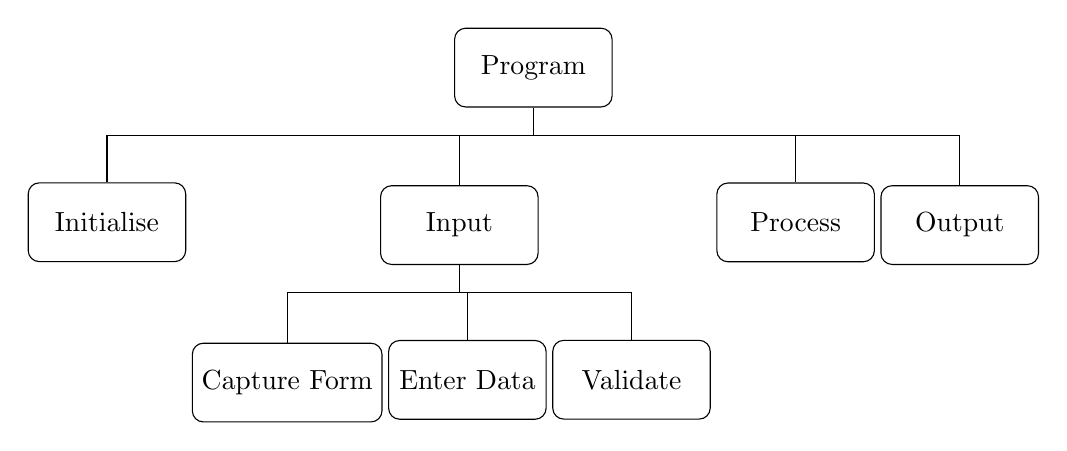
\begin{tikzpicture}[
				level 1/.append style={level distance=2cm},
				level 2/.append style={level distance=2cm}]
					\tikzstyle{every node}=[rectangle, rounded corners, minimum width=2cm, minimum height=1cm,text centered, draw=black]
					\Tree 
						[.Program
							[.{Initialise} ]
							[.{Input}
								[.{Capture Form} ]
								[.{Enter Data} ]
								[.{Validate} ]
							]
							[.{Process} ]
							[.{Output} ]
						]
				\end{tikzpicture}
			\end{figure}
			\noindent
			A flowchart is a diagram using standard symbols that describes a process or system. A system flowchart is a diagram that shows individual processes within a system. It often possible to create just one flowchart that shows the entire system, but this is not always a good idea as modern programs can be very large and putting every process on to one flowchart might make it too complex to be of any real use. This can be fixed by having multiple flowcharts for the multiple systems.\\
			Pseudo-code is a method of writing code that does not require knowledge of a particular programming language without having to worry about syntax or constructs. The only true rule of Pseudo-code is that it has to be internally consistent, for example if you write \verb|print| in one place and then write \verb|output|, this is considered bad practice and also makes it harder to convert it to a programming language later.\\
			Pseudo-code can be used at many levels of detail meaning it is up to the programmer to decide what level of detail is appropriate to the project they are planning to do. One of the major benefits of using Pseudo-code is it allows the programmer to see how his code may eventually be laid out.\\
			Naming Conventions is the process of giving meaningful names to subroutines, functions, variables and other user-defined features in a program. Before coding, a list of all the variables, including their data type and scope (Global or local) should be made. A similar procedure should also be carried out for all functions and subroutines to be featured within the program.\\
			When writing the actual code, you should try and make your program as programmer-friendly  as possible with the use of code layout and comments, examples of this would be:
			\begin{itemize}
				\setlength\itemsep{0cm}
				\item Comments to show the purpose of an algorithm.
				\item Comments to show the purpose of each line.
				\item Sensible variable names.
				\item Indenting the contents of loops and subroutines.
			\end{itemize}
			After the code is initially written, debugging will often have to occur. This can be done using a dry run and a trace table. A dry run is the process of stepping through each line of code to see what will happen before a program is run, a trace table is a method of recording the result of each step that takes place when dry running code.
	\section{Fundamentals of Data Structure}
		\subsection{Data Structures and Abstract Data Types}
			\marginnote{3.2.1.1}A data structure is any method used to store data in an organised and accessible format, they normally contain data that are related, different data structures allow for different data manipulations which means different data structures are use for different types of applications. For example an array may be useful to store a list of names whereas a textfile may be used to store information for a database.
			\marginnote{3.2.1.2}An array is a set of related data items stored under a single identifier, they can have one or more dimensions, all elements are often of the same type(homogeneous). An array most commonly has either one dimension(which can be useful to represent vectors) which can be visualised using a list, or two dimensions (which is useful for representing a matrix) which can be visualised using a two-dimensional table. In python, instead of Arrays we use lists, which have a few minute differences to standard arrays (python lists are heterogeneous(They can store dat of different types)) but can be used in the same way as arrays. Some uses of lists are as follows:
			\begin{lstlisting}[language=python]
Studentname = ["Derrick","Gill","Jamal","Lois"]
Studentname[1]
'Gill'

ArrayAdd=[[0,1,2],[1,2,3],[2,3,4]]
ArrayAdd[1][2]
3		\end{lstlisting}
			\marginnote{3.2.1.3}Files are used to store many different types of data meaning that many different file types are needed to store all of these different types of data. Many file types are portable meaning that they can be used on many different platforms, the two most common portable file types when programming are text files (which is a file that contains human readable characters) and binary files (which stores data as 1s and 0s). One line on a text file may be referred to as a record, and the different items of data stored within the record are called the fields.\\
			All files have an internal structure which allows them to store data efficiently, there are two common structures that are used to store data These are:\\
			Tab-delimited text (txt) file:
			\begin{lstlisting}
Sara	Phillips	sphillips0@google.co.jp	Female	117.135.192.97
Laura	Harvey	lharvey1@utexas.edu	Female	62.114.62.185
Eugene	Wells	ewells2@weibo.com	Male	119.176.45.229
Helen	Jordan	hjordan3@geocities.jp	Female	81.49.64.62
Shirley	Weaver	sweaver4@pbs.org	Female	218.20.41.34	\end{lstlisting}
			Comma seperate variable (csv):
			\begin{lstlisting}
Sara,Phillips,sphillips0@google.co.jp,Female,117.135.192.97
Laura,Harvey,lharvey1@utexas.edu,Female,62.114.62.185
Eugene,Wells,ewells2@weibo.com,Male,119.176.45.229
Helen,Jordan,hjordan3@geocities.jp,Female,81.49.64.62
Shirley,Weaver,sweaver4@pbs.org,Female,218.20.41.34 	\end{lstlisting}
			To read and write to csv, we can use the python module csv:
			\begin{lstlisting}[language=python]
import csv
file=open("Contacts.csv","a+",newline='')
Reader = csv.reader(file) # This reads the contents of the file
Writer = csv.writer(file) # This creates an object which allows us to write to the file.
file.write("\n")
Writer.writerow(['Joe', 'Shmuck', 'JShmuck3D@hotmail.com', 'Male','162.148.10.205'])
file.close()	\end{lstlisting}
			Binary files contain binary codes and usually contain some header information that describes what these represent, binary files are not easily readable by a human, but can quickly be interpreted by a program. For example, the PNG image file is a binary file, can be used in a range of applications and requires less memory than some other image formats. Many program files (executables) are binary files so they can be used on other platforms. The two main actions you might want to perform on binary files are to read and write data from and to it.
	\section{Systematic Approach to Problem Solving}
		\subsection{Aspects of Software Development}
			\begin{tikzpicture}
			
			\def \n {3}
			\def \radius {5cm}
			\def \margin {8} % margin in angles, depends on the radius
			\def \x {1}
			
			\foreach \s in {a,b,c}
			{
				\node[draw, circle] at ({360/\n * (\x - 1)}:\radius) {\s};
				\draw[->, >=latex] ({360/\n * (\x - 1)+\margin}:\radius) 
				arc ({360/\n * (\x - 1)+\margin}:{360/\n * (\x)-\margin}:\radius);
				\def \x {\x + 1}
			}
			\end{tikzpicture}
\end{document}